\chapter{Applications}
In this chapter we will discuss an example of a place where Quantum Homomorphic Encryption can be used.
 
\section{The Airport Example}
\subsection{Problem Definition}
We want to detect unauthorized personnel accessing distinguished places in the airport. We do not trust the server since it can be interfered with and information changed hence we are unable to detect the unauthorized personnel. The server may also decide to be malicious and relay the wrong information. 

\subsection{Requirements}
We will require Closed Circuit Television (CCTV) cameras, a client who is classical and requires to request services of a quantum computer.

\subsection{How it works}
The CCTV cameras relay images to the client on real time. The client encrypts the face images received. The encrypted images are sent to the server. The server has the face images of authorized persons which are also encrypted. The server performs face recognition on the encrypted images. The server knows the computation it is performing since in Homomorphic Encryption the computation is not encrypted. If an image does not match the images they have, then an encrypted intrusion message is produced. The server does not know what the output is. The message is sent to the doors and the security. The doors are supposed to automatically close and the security is supposed to immediately appear on the scene.

If a message is only sent when an intruder is detected then this may reveal some information to the server. A message has to be sent to the doors and security all the time. In case no intruder is detected then the doors should remain open and the security should not appear.  

The CCTV should also be placed in locations where a face can be clearly captured and is unknown to the public since some clever people may decide to interfere with it. The output of the server should not also be a single quantum bit for example $|0 \rangle$ when an intruder is detected and $|1\rangle$ for an authorized personnel. This same clever person could flip the bit when it is being relayed. As we saw earlier, a quantum state cannot be cloned because cloning involves measurement and measurement changes the state.  

\subsection{Why does the client require services of the server in this example}
An airport is automatically large and the number of authorized personnel in different departments and sections are also many. The client requires storage facilities. The client does not have the capability of performing face recognition on a very large number of images. This computation requires high processing power and speed which the client does not possess. 

Fig \ref{fig2: The Airport Model} shows the model

\begin{figure}[h]
\center
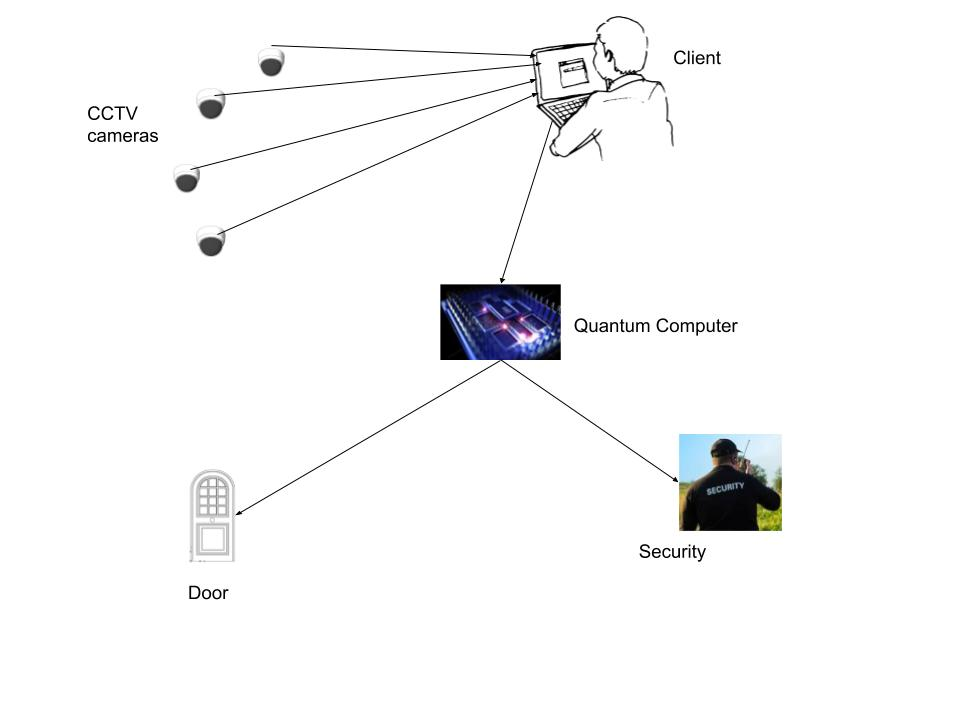
\includegraphics[scale=0.5]{images/Model2.jpg}
\caption{The Airport Model} 
\label{fig2: The Airport Model}
\end{figure}

\newpage
\subsection{Assumptions made in this model}
There are few assumptions made while building this model. The server has the ability to perform face recognition on encrypted face images. Since the output options are two, whether an authorized person or an intruder then different encryptions to represent each of them are produced at different times.

\subsection{Algorithm}  
Figure \ref{fig3 : algorithm} is an algorithm of how the model works.
The client generates both public and private using Rivest-Shamir-Adleman (RSA) method. The public key is used to encrypt the images before they are sent to the quantum server for storage. The client then receives images relayed by the camera and encrypts them one by one. The encrypted images relayed are then sent to the quantum server to perform face recognition. The quantum server performs the face recognition on the encrypted images. If the face image matches any of the encrypted images stored, then a message is sent to the doors to remain open and to the security not to act. If the image does not match any of the images stored then a message that doors should close and security should go to the scene is sent. 
\begin{figure}[!h]
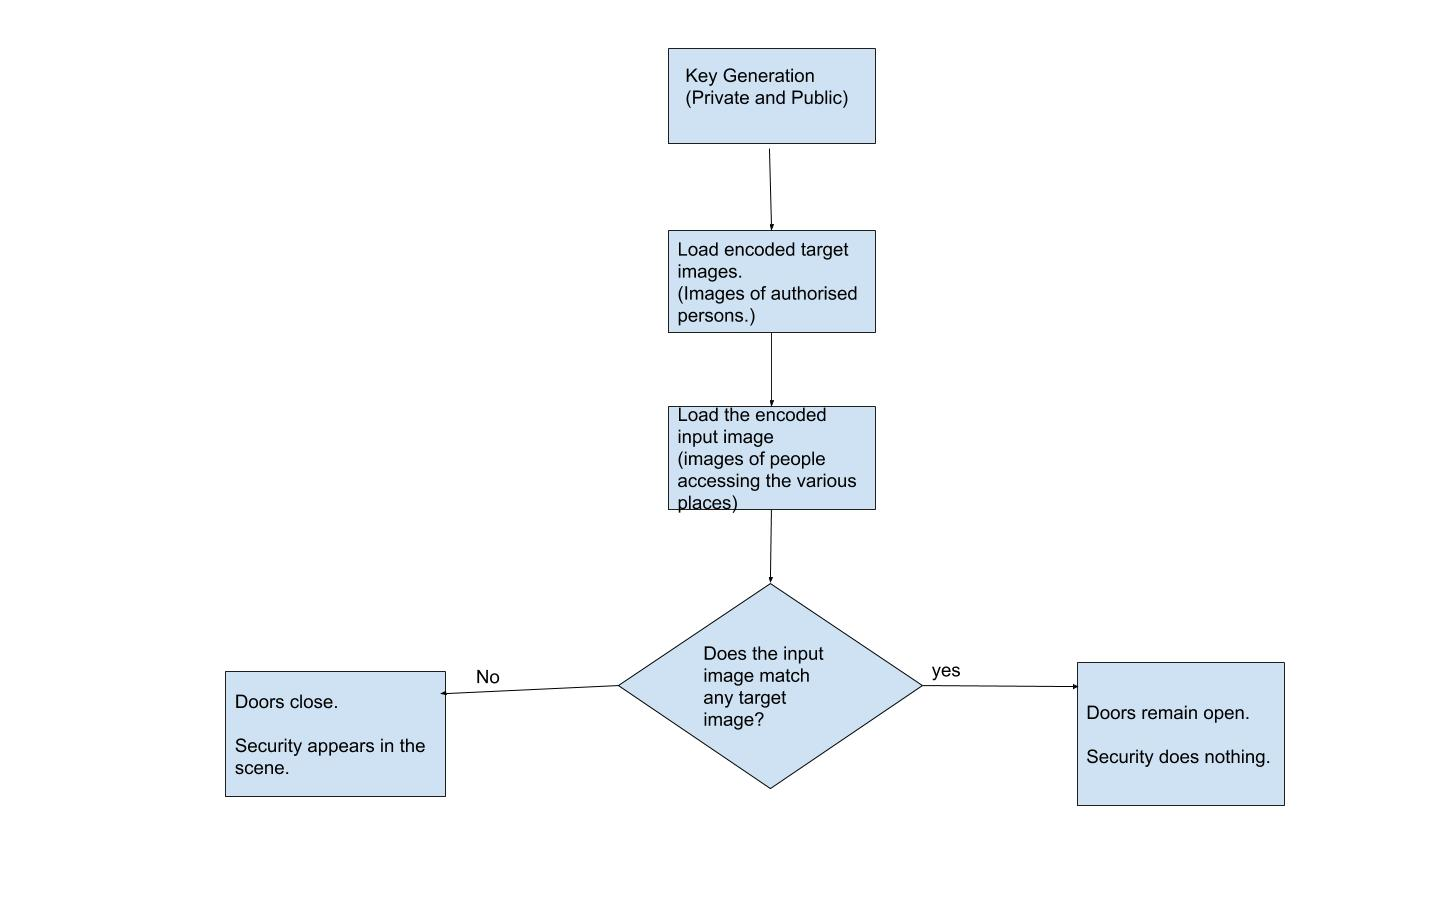
\includegraphics[scale=0.375]{images/Algorithm.jpg} 
\caption{Algorithm}
\label{fig3 : algorithm}
\end{figure}
\newpage
\subsection{How the python code for the model works}
The following is a python code using face recognition module in Python (Python Code in Appendix). The code uses two images. One is the image of the authorized personnel while the other is relayed image. In the code the images are not encrypted but we assume in the quantum server they are encrypted. The program uses RSA a module that produces a private key and public key. The public key encrypts the message and the private key decrypts it. In the code the output is encrypted after performing face recognition. The encrypted code is the sent to the classical client operating the doors and to the security. They are prompted to enter their private codes known only to them. The message is then decrypted and they can act accordingly. In case a wrong code is entered then two more chances are given after which the system automatically blocks.

\subsection{Sample outputs using the python code}
For the case where the input face image matches with the target face image.
\begin{figure}
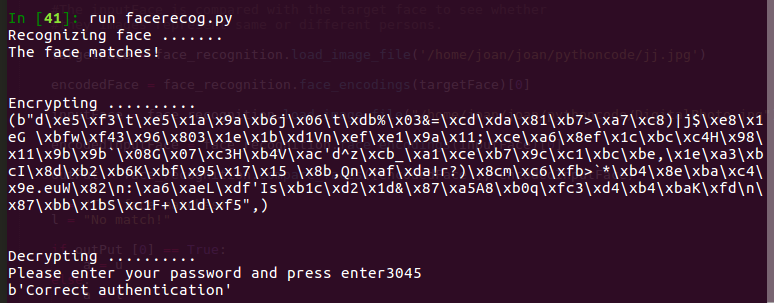
\includegraphics[scale=0.5]{images/facematch.png} 
\caption{Face match}
\label{fig4: Output when the images match.}
\end{figure}
Correct authentication implies that doors should remain open and the security should not appear anyway Fig \ref{fig4: Output when the images match.}.

For the case where the input face does not match with the target face image.
\begin{figure}
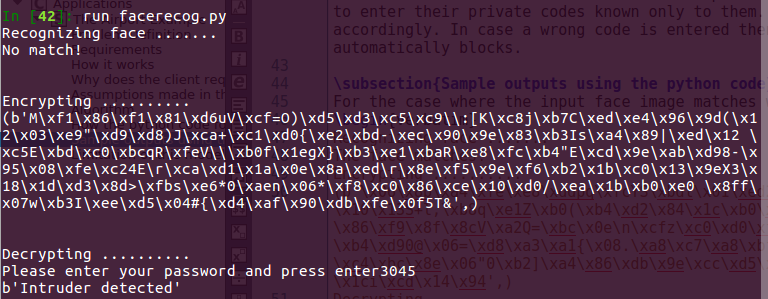
\includegraphics[scale=0.5]{images/Nomatch.png} 
\caption{No Match}
\label{fig5 :  Output when the images do not match.}
\end{figure}
Intruder detected implies that doors should close and the security should appear in the scene
Fig \ref{fig5 :  Output when the images do not match.}.

\subsection{Limitation of this model}
This model poses one major limitation which is very vital. In case a wrong code is entered three times the system automatically blocks. This implies that the required action is not taken for example doors closing. If does are not closed the intruder may get away before the security get to the specific location.  


